\chapter{Milestone reports}
\label{app:Milestone-Reports}
This chapter lists the individual milestone reports. These should provide information on the status of the project during realisation. For every completed milestone, a report was written before the next phase could be started. The table \fullref{tab:Milestones} shows the milestones within the thesis as well as the dates when the milestone and the phase will be completed and reviewed. The milestones are also shown in the whole project plan in \fullref{fig:Project-Plan}.

\section{Milestone report M1 from the 15.03.2020}

\subsection{What work was carried out in the last reporting period}

\subsection{State of progress}

\subsection{Top three risks including planned measures}

\chapter{SINS database table}
\label{app:SINS-Databse-Table}
This chapter shows a table with the different activities recorded within the SINS database. The activites are divided into the room where they were recorded.

\begin{table}[htbp]
    \centering
    \caption[SINS database recorded activities for each room]{SINS database recorded activities for each room \footnotemark}
	\label{tab:sins-database-recorded-activities}
    \begin{tabular}{l|l|c|c}
        \toprule
        \textbf{Room} & \textbf{Activity} & \textbf{Nr. ex.} & \textbf{duration (min.)} \\ 
        \midrule[1pt]
        \multirow{10}{*}{Living room} & Phone call & 22 & 8.17 $\pm$ 13.73 \\
        \cline{2-4}
        & Cooking & 19 & 16.62 $\pm$ 9.49 \\
        \cline{2-4}
        & Dish washing & 15 & 6.37 $\pm$ 1.49 \\
        \cline{2-4}
        & Eating & 19 & 7.78 $\pm$ 4.27 \\
        \cline{2-4}
        & Visit & 9 & 13.3 $\pm$ 12.11 \\
        \cline{2-4}
        & Watching TV & 13 & 155.38 $\pm$ 93.28 \\
        \cline{2-4}
        & Working & 15 & 31.24 $\pm$ 39.33 \\
        \cline{2-4}
        & Vacuum cleaning & 15 & 4.79 $\pm$ 2.14 \\
        \cline{2-4}
        & Other & 15 & 0.75 $\pm$ 0.95 \\
        \cline{2-4}
        & Absence & 15 & 66.37 $\pm$ 130.30 \\
        \midrule[1pt]
        \multirow{7}{*}{Bathroom} & Drying with towel & 10 & 1.67 $\pm$ 0.28 \\
        \cline{2-4}
        & Shaving & 13 & 1.91 $\pm$ 1.46 \\
        \cline{2-4}
        & Showering & 10 & 6.11 $\pm$ 2.38 \\
        \cline{2-4}
        & Tooth brushing & 19 & 1.41 $\pm$ 0.25 \\
        \cline{2-4}
        & Vacuum cleaning & 9 & 0.87 $\pm$ 0.59 \\
        \cline{2-4}
        & Other & 75 & 0.42 $\pm$ 0.4 \\
        \cline{2-4}
        & Absence & 35 & 248.56 $\pm$ 263.62 \\
        \midrule[1pt]
        \multirow{3}{*}{Hall} & Vacuum cleaning & 9 & 3.31 $\pm$ 1.11 \\
        \cline{2-4}
        & Other & 164 & 0.36 $\pm$ 0.22 \\
        \cline{2-4}
        & Absence & 175 & 50.17 $\pm$ 102.52 \\
        \midrule[1pt]
        \multirow{3}{*}{Toilet} & Toilet visit & 21 & 4.74 $\pm$ 3.24 \\
        \cline{2-4}
        & Vacuum cleaning & 7 & 0.53 $\pm$ 0.07 \\
        \cline{2-4}
        & Absence & 31 & 282.75 $\pm$ 263.19 \\
        \midrule[1pt]
        \multirow{5}{*}{Bedroom} & Dressing & 28 & 1.53 $\pm$ 1.10 \\
        \cline{2-4}
        & Sleeping & 7 & 348.43 $\pm$ 130.73 \\
        \cline{2-4}
        & Vacuum cleaning & 7 & 1.04 $\pm$ 0.27 \\
        \cline{2-4}
        & Other & 22 & 0.27 $\pm$ 0.23 \\
        \cline{2-4}
        & Absence & 22 & 122.28 $\pm$ 157.43 \\
        \bottomrule
    \end{tabular}
\end{table}
\footnotetext{\fullcite{dekkers_sins_2017}}

\chapter{Work journal}
\label{app:Work-Journal}

Within this chapter, the whole work journal of the thesis is shown. The journal is divided into subcategories, so that the \fullref{tab:Work-Journal} is more pleased to read. These categories show what exactly was done in the different project phases, which can be seen in the \fullref{fig:Project-Plan}. There is also one more category called \flqq General\frqq, where all the administrative tasks are shown, including the meetings with the advisor.

\clearpage
\landscapevalues

\begin{longtable}{| p{.10\textwidth} | p{.20\textwidth} | p{.50\textwidth} | p{.10\textwidth} |} 
	\caption{Work Journal}
	\label{tab:Work-Journal} \\
    \hline
    \textbf{Date} &
    \textbf{Task} &
    \textbf{Details} &
    \textbf{No. hours} \\
    \hline
    \multicolumn{4}{|l|}{\textbf{General}} \\
    \hline
    17.02.2020 & Preparation for Kick-Off Meeting & 
        \begin{minipage}{5in}
        \vskip 4pt
        \begin{itemize}
        \setlength\itemsep{0em}
        \item thesis description read carefully again
        \item questions of unclear matters
        \end{itemize}
        \vskip 4pt
        \end{minipage}
        & 1h  \\
    \hline
    17.02.2020 & Kick-Off Meeting (number 1)& 
        \begin{minipage}{5in}
        \vskip 4pt
        \begin{itemize}
        \setlength\itemsep{0em}
        \item discussed different topics which are important for the implementation of the project
        \end{itemize}
        \vskip 4pt
        \end{minipage}
        & 1h 30min  \\
    \hline
    24.02.2020 & Meeting (number 2) & 
        \begin{minipage}{5in}
        \vskip 4pt
        \begin{itemize}
        \setlength\itemsep{0em}
        \item preparation of the meeting
        \item meeting itself
        \end{itemize}
        \vskip 4pt
        \end{minipage}
        & 2h  \\
    \hline
    02.03.2020 & Meeting (number 3) & 
        \begin{minipage}{5in}
        \vskip 4pt
        \begin{itemize}
        \setlength\itemsep{0em}
        \item preparation of the meeting
        \item meeting itself
        \end{itemize}
        \vskip 4pt
        \end{minipage}
        & 2h  \\
    \hline
    02.03.2020 & Meeting GPU with Thomas Koller & 
        \begin{minipage}{5in}
        \vskip 4pt
        \begin{itemize}
        \setlength\itemsep{0em}
        \item preparation of the meeting
        \item meeting itself
        \end{itemize}
        \vskip 4pt
        \end{minipage}
        & 0.5h  \\
    \hline
    09.03.2020 & Meeting (number 4) & 
        \begin{minipage}{5in}
        \vskip 4pt
        \begin{itemize}
        \setlength\itemsep{0em}
        \item preparation of the meeting
        \item meeting itself
        \end{itemize}
        \vskip 4pt
        \end{minipage}
        & 2h  \\
    \hline
    \multicolumn{4}{|l|}{\textbf{Documentation}} \\
    \hline
    17.02.2020 & Documentation setup & 
        \begin{minipage}{5in}
        \vskip 4pt
        \begin{itemize}
        \setlength\itemsep{0em}
        \item project setup
        \item latex document setup
        \item German transcribed to English
        \item built default documentation structure
        \end{itemize}
        \vskip 4pt
        \end{minipage}
        & 2h  \\
    \hline
    19.02.2020 & Dataset documented & 
        \begin{minipage}{5in}
        \vskip 4pt
        \begin{itemize}
        \setlength\itemsep{0em}
        \item SINS Database
        \item DCASE Task dataset
        \end{itemize}
        \vskip 4pt
        \end{minipage}
        & 3h  \\
    \hline
    24.02.2020 & Dataset section finished & 
        \begin{minipage}{5in}
        \vskip 4pt
        \begin{itemize}
        \setlength\itemsep{0em}
        \item Created table of the recorded activities in the \gls{SINS} database
        \item Reread section and corrected
        \end{itemize}
        \vskip 4pt
        \end{minipage}
        & 1h  \\
    \hline
    02.03.2020 & Triplet Loss section finished & 
        \begin{minipage}{5in}
        \vskip 4pt
        \begin{itemize}
        \setlength\itemsep{0em}
        \item Documented Triplet Loss in related work
        \item Reread section and corrected
        \end{itemize}
        \vskip 4pt
        \end{minipage}
        & 2h  \\
    \hline
    03.03.2020 & Tile2Vec section finished & 
        \begin{minipage}{5in}
        \vskip 4pt
        \begin{itemize}
        \setlength\itemsep{0em}
        \item Documented Tile2Vec in related work
        \item Reread section and corrected
        \item Corrected equations
        \end{itemize}
        \vskip 4pt
        \end{minipage}
        & 2h  \\
    \hline
    05.03.2020 & Started with intro to neural networks & 
        \begin{minipage}{5in}
        \vskip 4pt
        \begin{itemize}
        \setlength\itemsep{0em}
        \item Researched neural networks
        \item Documented neural networks
        \end{itemize}
        \vskip 4pt
        \end{minipage}
        & 4h  \\
    \hline
    06.03.2020 & Finished with intro to neural networks & 
        \begin{minipage}{5in}
        \vskip 4pt
        \begin{itemize}
        \setlength\itemsep{0em}
        \item Documented neural networks
        \end{itemize}
        \vskip 4pt
        \end{minipage}
        & 4h  \\
    \hline
    05.03.2020 & Started with intro to convolutional neural networks & 
        \begin{minipage}{5in}
        \vskip 4pt
        \begin{itemize}
        \setlength\itemsep{0em}
        \item Researched convolutional neural networks
        \item Documented convolutional neural networks
        \end{itemize}
        \vskip 4pt
        \end{minipage}
        & 2h  \\
    \hline
    09.03.2020 & Finished intro to convolutional neural networks & 
        \begin{minipage}{5in}
        \vskip 4pt
        \begin{itemize}
        \setlength\itemsep{0em}
        \item Documented convolutional neural networks
        \end{itemize}
        \vskip 4pt
        \end{minipage}
        & 3h  \\
    \hline
    09.03.2020 & Documented various parts & 
        \begin{minipage}{5in}
        \vskip 4pt
        \begin{itemize}
        \setlength\itemsep{0em}
        \item Documented project plan and milestones
        \item Documented introduction
        \item Documented appendix
        \item Documented into to clustering
        \end{itemize}
        \vskip 4pt
        \end{minipage}
        & 3h  \\
    \hline
    11.03.2020 & Document changes applied from meeting & 
        \begin{minipage}{5in}
        \vskip 4pt
        \begin{itemize}
        \setlength\itemsep{0em}
        \item Moving Dataset to related work
        \item Changed denotation of loss function
        \item Changed NN section
        \end{itemize}
        \vskip 4pt
        \end{minipage}
        & 1h  \\
    \hline
    11.03.2020 & Finished intro to gated recurrent unit & 
        \begin{minipage}{5in}
        \vskip 4pt
        \begin{itemize}
        \setlength\itemsep{0em}
        \item Documented gated recurrent unit
        \end{itemize}
        \vskip 4pt
        \end{minipage}
        & 2h  \\
    \hline
    13.03.2020 & Finished status in relation to project & 
        \begin{minipage}{5in}
        \vskip 4pt
        \begin{itemize}
        \setlength\itemsep{0em}
        \item Researched state-of-the-art in audio deep learning
        \item Documented status in relation to project
        \end{itemize}
        \vskip 4pt
        \end{minipage}
        & 4h  \\
    \hline
    \multicolumn{4}{|l|}{\textbf{Research}} \\
    \hline
    17.02.2020 & Research Dataset & 
        \begin{minipage}{5in}
        \vskip 4pt
        \begin{itemize}
        \setlength\itemsep{0em}
        \item finished with DCASE - Challenge description
        \item started with SINS Database Paper
        \end{itemize}
        \vskip 4pt
        \end{minipage}
        & 2h 30min  \\
    \hline
    21.02.2020 & Audio processing research & 
        \begin{minipage}{5in}
        \vskip 4pt
        \begin{itemize}
        \setlength\itemsep{0em}
        \item \gls{FT}
        \item \gls{FFT}
        \item \gls{DFT}
        \item Spectrogram
        \item started with related work documentation
        \end{itemize}
        \vskip 4pt
        \end{minipage}
        & 5h  \\
    \hline
    26.02.2020 & Audio processing research & 
        \begin{minipage}{5in}
        \vskip 4pt
        \begin{itemize}
        \setlength\itemsep{0em}
        \item \gls{MFCC}
        \item documenting research in related work
        \end{itemize}
        \vskip 4pt
        \end{minipage}
        & 3h  \\
    \hline
    27.02.2020 & Audio processing research & 
        \begin{minipage}{5in}
        \vskip 4pt
        \begin{itemize}
        \setlength\itemsep{0em}
        \item \gls{MFCC}
        \item finished documenting research in related work
        \end{itemize}
        \vskip 4pt
        \end{minipage}
        & 4h  \\
    \hline
    28.02.2020 & Triplet Loss research & 
        \begin{minipage}{5in}
        \vskip 4pt
        \begin{itemize}
        \setlength\itemsep{0em}
        \item read various paper on triplet loss
        \end{itemize}
        \vskip 4pt
        \end{minipage}
        & 3h  \\
    \hline
    01.03.2020 & Triplet Loss research & 
        \begin{minipage}{5in}
        \vskip 4pt
        \begin{itemize}
        \setlength\itemsep{0em}
        \item current research on triplet loss with audio
        \end{itemize}
        \vskip 4pt
        \end{minipage}
        & 2h  \\
    \hline
    02.03.2020 & Tile2Vec research & 
        \begin{minipage}{5in}
        \vskip 4pt
        \begin{itemize}
        \setlength\itemsep{0em}
        \item read various paper on tile2vec
        \item started documenting tile2vec in related work
        \end{itemize}
        \vskip 4pt
        \end{minipage}
        & 5h  \\
    \hline
\end{longtable}

\clearpage
\defaultpagestyle

\chapter{Task definition bachelor thesis}
\label{app:Task-Definition}

Within this chapter the final task definition, which was submitted and accepted by the Transfer Office of the Lucerne University of Applied Sciences and Arts on the 25.02.2020, is attached.

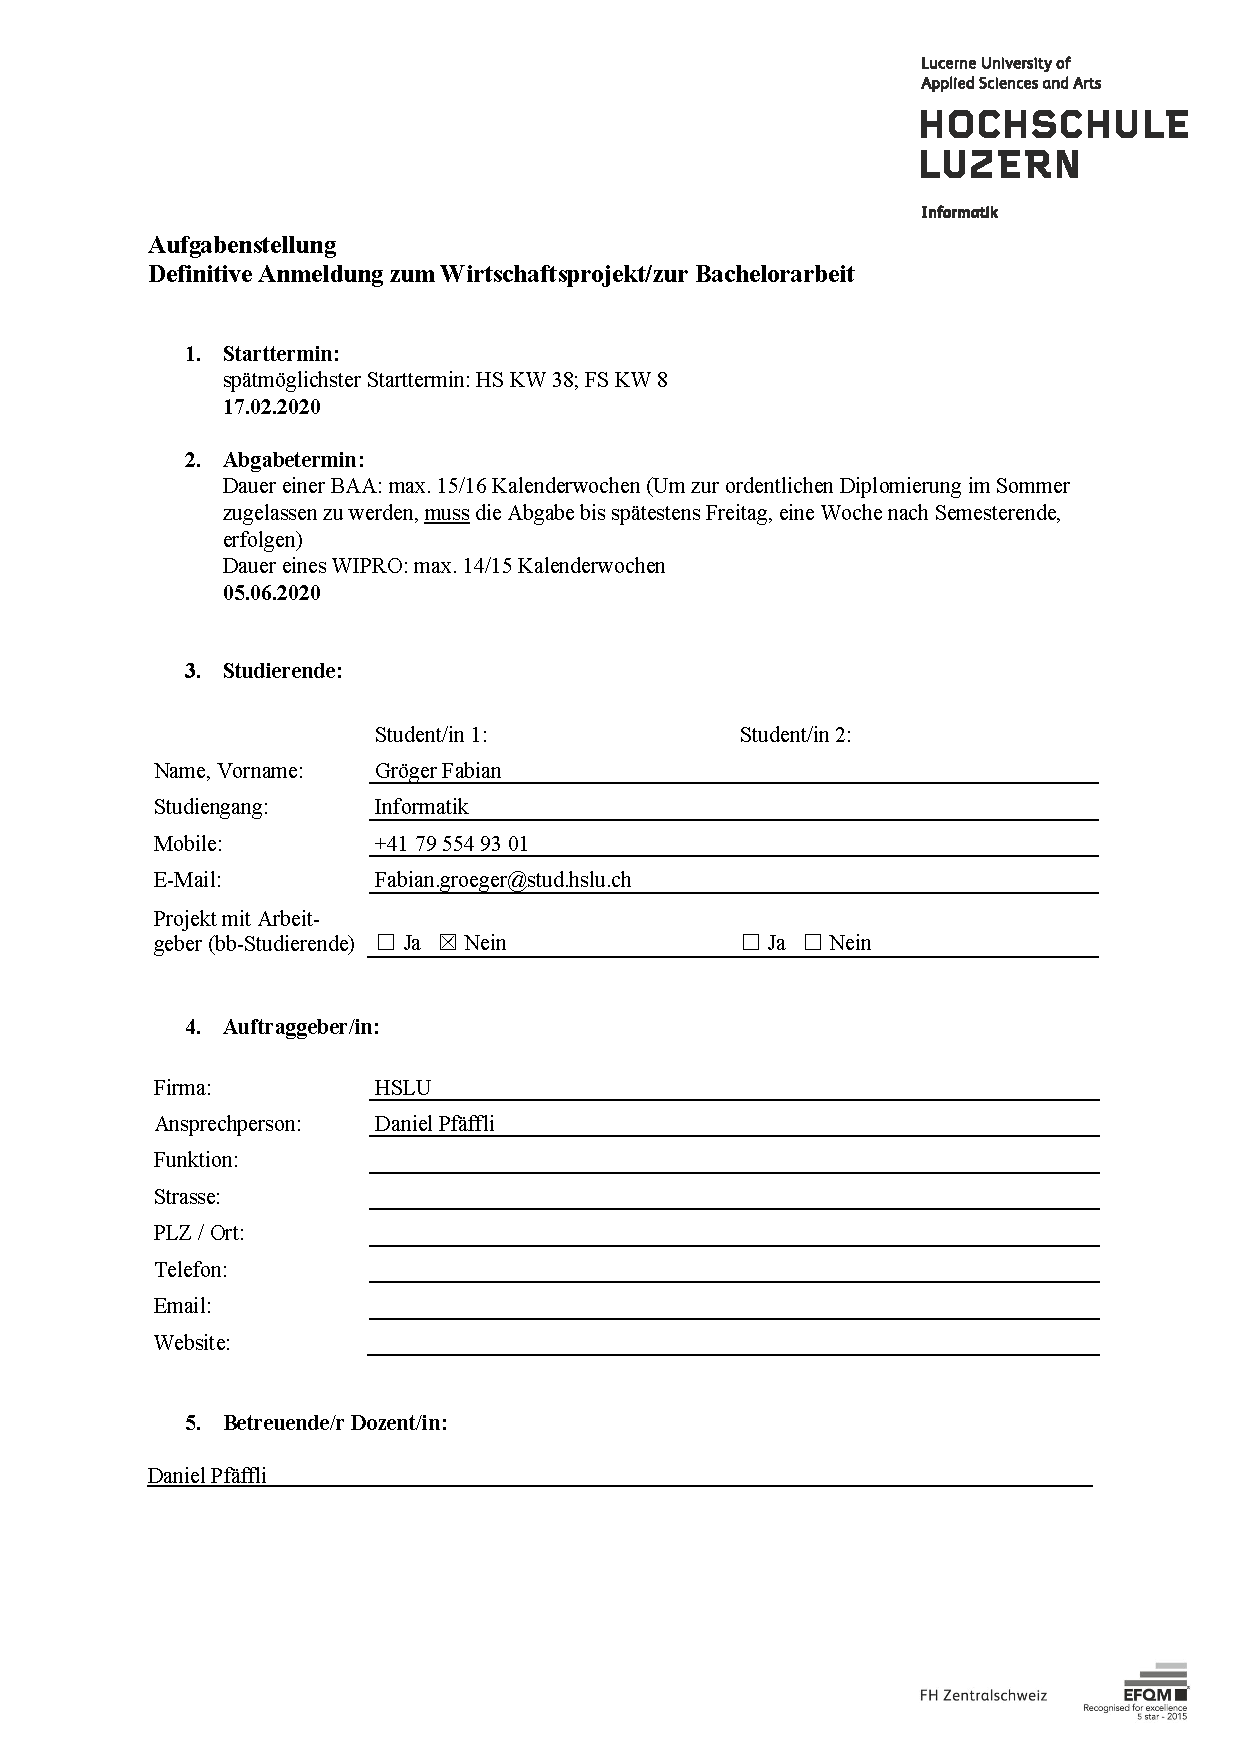
\includepdf[scale=0.9, pages=1-]{files/Aufgabenstellung_DeepEmbeddedMusic.pdf}
